
\documentclass[a4paper,12pt]{report}
\usepackage {xcolor}
\usepackage {color}
\usepackage[unicode]{hyperref}
\usepackage[nottoc,numbib]{tocbibind}
\hypersetup{colorlinks=true, urlcolor=green, linkcolor=black, unicode=true}
\usepackage[utf8]{inputenc}
\usepackage[utf8]{vietnam}
\usepackage{latexsym, amsfonts, amssymb, amsmath}
\usepackage[margin=2.2cm]{geometry}
\usepackage{fancybox}
\usepackage{minted}
\usepackage{frame}
\usepackage{framed}
\usepackage{graphicx}

\usepackage{tikz}
\usepackage{tikz-cd}
\usetikzlibrary{matrix}
\usetikzlibrary{automata,arrows,positioning,matrix,calc}

\newcommand{\mnt}[1]{\inputminted[frame=single, linenos=true, tabsize=4]{c++}{#1}}

\begin{document}
\thispagestyle{empty}
\thisfancypage{
\setlength{\fboxsep}{0pt}
\fbox}{} 
\begin{center}
    \begin{large}
        \textcolor[rgb]{1.00,0.00,0.00}{TRƯỜNG ĐẠI HỌC BÁCH KHOA HÀ NỘI}
    \end{large} \\
    \begin{large}
        \textcolor[rgb]{1.00,0.00,0.00}{VIỆN CÔNG NGHỆ THÔNG TIN VÀ TRUYỀN THÔNG}
    \end{large} \\

    \textbf{--------------------  *  ---------------------}\\[2cm]

    
\includegraphics[width=3cm, height=4.2cm]{img/logo.jpg}\\[1cm]
    {\fontsize{32pt}{1}\selectfont ĐỒ ÁN I}\\
    {\fontsize{20pt}{1}\selectfont LẬP TRÌNH}\\[2cm]
\end{center}


\begin{flushright}
    \parbox[t]{10cm}{
    \textbf{Phạm Văn Thông}\\MSSV: 20136495\\}
\end{flushright}

\hspace{5cm} Giáo viên hướng dẫn\hspace{24pt} :
\begin{flushright} \textbf{\parbox[t]{8cm}{    
        \textcolor[rgb]{0.00,0.00,1.00}{Phạm Đăng Hải}
        }}
\end{flushright}
    \vspace{2cm}
\begin{center}
        {\fontsize{16pt}{1}\selectfont HÀ NỘI}\\
        {\fontsize{16pt}{1}\today}
\end{center}

\newpage
\abstract
Báo cáo gồm ba phần trình bày các bài toán sắp xếp, giải thuật quay lui, đánh chỉ mục từ khóa trong văn bản. 
Phần thứ nhất trình bày về ý tưởng, cài đặt và độ phức tạp của các thuật toán sắp xếp cơ bản bao gồm \texttt{buble sort, selection sort, insertion sort, shell sort, quick sort, heap sort}. Phần thứ hai trình bày một số bài toán về giải thuật quay lui trong bài toán \emph{tám hậu}, \emph{mã đi tuần} và kĩ thuật nhánh cận trong bài toán \emph{người du lịch}. Phần thứ ba trình bày về các cách cài đặt khác nhau của bài toán đánh chỉ mục từ khóa trong văn bản trên các cấu trúc dữ liệu khác nhau bao gồm \emph{danh sách liên kết}, \emph{bảng băm}, \emph{cây nhị phân tìm kiếm}

Các chương trình trong báo cáo được trình bày bằng ngôn ngữ lập trình C++
\section{Các thuật toán sắp xếp}
\subsection{Bài toán sắp xếp}

Sắp xếp là quá trình bố trí lại các phần tử của một tập đối tượng nào đó theo một thứ tự nhất định. Chẳng hạn như thử tự tăng dần (hay giảm dần) đối với một dãy số, thứ tự từ điển đối với các từ v.v... Yêu cầu về sắp xếp thường xuyên xuất hiện trong các ứng dụng Tin học với các mục đích khác nhau: sắp xếp dữ liệu trong máy tính để tìm kiếm cho thuận lợi, sắp xếp các kết quả xử lý để in ra trên bảng biểu v.v...

Nói chung dữ liệu có thể xuất hiện dưới nhiều dạng khác nhau. Một tập các đối tượng cần được sắp xếp là tập các bản ghi (records), mỗi bản ghi bao gồm một số trường (fields) khác nhau. Nhưng không phải toàn bộ mà chỉ là một trương nào đó (hay một vài trường nào đó được chú ý tới thôi. Trường như vậy chúng ta gọi là là \textsf{khóa} (textsf{key}). Sắp xếp sẽ được tiến hành dựa vào giá trị của khóa này.\\

Khi sắp xếp, các bản ghi trong bảng sẽ được đặt vào các vị trí sao cho các giá trị khóa tương ứng của chúng có đúng thứ tự đã ấn định. thì kích thước của toàn bản ghi có thể rất lớn, nên
nếu việc sắp xếp thực hiện trực tiếp trên các bản ghi sẽ đòi hỏi sự chuyển đổi vị trí của các
bản ghi, kéo theo việc thường xuyên phải di chuyển, copy những vùng nhớ lớn, gây ra những
tổn phí thời gian khá nhiều. Thường người ta khắc phục tình trạng này bằng cách xây dựng
một bảng khoá: Mỗi bản ghi trong bảng ban đầu sẽ tương ứng với một bản ghi trong \textsf{bảng
khoá}. Bảng khoá cũng gồm các bản ghi nhưng mỗi bản ghi chỉ gồm có hai trường: 
\begin{itemize}
\item Trường thứ nhất chứa khóa.
\item Trường thứ hai chứa liên kết tới một bản ghi trong bảng ban đầu, tức là một thông tin đủ để biết bản ghi tương ứng với nó trong bảng ban đầu là bản ghi nào.
\end{itemize}

Có thể coi \emph{khóa như là đại diện cho các bản ghi} và để đơn giản, ta chỉ nói tới giá trị khóa mà thôi. Các thao tác trong kĩ thuật sắp xếp lẽ ra là tác động lên toàn bản ghi giờ đây chỉ làm việc trên khóa.

\subsection{Một số quy ước}
Mục này trình bày các cài đặt một số giải thuật sắp xếp phổ biến. Để thuận tiện hơn trong việc theo dõi chương trình sau này, ta đưa vào một số quy ước như sau:\\
\begin{itemize}
\item Dãy khóa cần được sắp xếp được lưu trong mảng \texttt{arr} gồm các phần tử từ $0...len-1$, trong đó, \texttt{len} là số phần tử của mảng.
\item hàm \texttt{swap(a, b)} có tác dụng đổi chỗ hai phần tử \texttt{a} và \texttt{b}
\item Kí hiệu arr[i...j] được hiểu là các phần tử từ arr[i] đến arr[j] trong mảng arr.
\end{itemize}



\subsection{Thuật toán sắp xếp nổi bọt}

Trong thuật toán săp xếp nổi bọt, các dãy khóa sẽ được duyệt từ cuối dãy lên đàu dãy (từ \texttt{arr[len-1]} về \texttt{arr[0]}), nếu gặp hai khóa kề nhau bị ngược thứ tự thì đổi chỗ của chúng cho nhau, sau lần duyệt như vậy, khóa nhỏ nhất sẽ trở về vị trí đầu tiên, quá trình lại tiếp tục với các khóa từ dãy \texttt{arr[1]} tới \texttt{arr[len-1]}:

\paragraph{Cài đặt}
Cài đặt thuật toán trong C++ như sau:
\mnt{src/bublesort.cpp}

\paragraph{Đánh giá độ phức tạp thuật toán}
Chọn phép toán so sánh $arr[i] < arr[j]$ làm phép toán tích cực để đánh giá hiệu suất thực hiện của thuật toán \emph{về mặt thời gian}. Ở lượt chọn thứ $i$ thì cần $n-i$ phép so sánh ($n$ là \emph{kích thước dữ liệu đầu vào}, trong trường hợp này $n = len$. Vậy số lần thực hiện phép so sánh là:
$$(n-1) + (n-2) + ... + 1 = \frac{n(n-1)}{2}$$. Vậy thời gian thực hiện của thuật toán là $O(n^2)$





\subsection{Thuật toán sắp xếp chọn}

Một trong những thuật toán sắp xếp đơn giản nhất là phương pháp sắp xếp chọn. Ý tưởng của thuật toán:
\begin{itemize}
\item Trong lần duyệt đầu tiên, duyệt dãy từ [0...len-1] tìm ra phần tử có giá trị nhỏ nhất đổi vị trí về đầu dãy.
\item Trong lần duyệt thứ k duyệt dãy từ [k-1...len-1] tìm ra phần tử tử nhỏ nhất trong dãy và đổi về vị trí k-1.
\item ...
\item Trong lần duyệtthứ \texttt{len}-1 chọn trong hai khóa \texttt{arr[len-2]} và \texttt{arr[len-1]} đổi với vị trí \texttt{len-2}
\end{itemize}

Kết thúc quá trình duyệt thì dãy còn lại đã được sắp xếp.

\paragraph{Cài đặt}
Sau đây là cài đặt của thuật toán trên C++:
\mnt{src/selectionsort.cpp}

\paragraph{Đánh giá độ phức tạp thuật toán}
Tương tự như giải thuật \emph{buble sort}, chọn phép toán $arr[i] < arr[min]$ làm phép toán tích cực để đánh giá độ phức tạp của thuật toán về mặt thời gian. Số lần thực hiện phép toán tích cực tương tự như đối với giải thuật \emph{buble sort} vẫn là $\frac{n(n-1)}{2} = O(n^2)$.





\subsection{Thuật toán sắp xếp kiểu chèn}

Xét dãy khóa arr[0...len-1], ta thấy chỉ gồm một khóa arr[0] chỉ gồm 1 khóa và có thể coi là đã sắp xếp rồi. Xét thêm arr[1], ta so sánh nó với arr[0], nếu thấy arr[1]<arr[0] thì ta chèn nó vào trước arr[1],... Một cách tổng quát, ta sẽ sắp xếp dãy arr[0...i-1] trong điều kiện dãy khóa đã được sắp xếp rồi chèn arr[i] vào dãy đó tại đúng vị trí để được dãy arr[0...i] đã được sắp xếp.

\paragraph{Cài đặt}
\mnt{src/insertionsort.cpp}

\paragraph{Đánh giá độ phức tạp thuật toán}
Đối với thuật toán sắp xếp kiểu chèn, thì chi phí thời gian thực hiện thuật toán phụ thuộc vào
tình trạng dãy khoá ban đầu. Nếu coi phép toán tích cực ở đây là phép so sánh $arr[i] > tmp$ thì:

\begin{itemize}
\item Trường hợp tốt nhất, ứng với dãy khóa đã sắp xếp rồi, mỗi lượt chỉ cần thực hiện một phép so sánh, như vậy, tổng số phép so sánh cần thực hiện là $n-1$. Phân tích trong trường hợp tốt nhất, độ phức tạp của thuật toán \emph{Insertion Sort} là $\Theta{n}$.
\item Trường hợp tồi nhất ứng với dãy khóa đã có thứ tự ngược lại, ở lượt sắp xếp thứ $i$ cần thực hiện $i-1$ phép so sánh. Số phép so sánh cần thực hiện là:
$$(n-1) + (n-2) + ... +1 = \frac{n(n-1)}{2}$$
Vậy thời gian thực hiện của thuật toán trong trường hợp tồi nhất là $O(n^2)$.
\item Trong trường hợp các khóa xuất hiện một cách ngẫu nhiên, có thể coi lượt thứ $i$ cần thực hiện $i/2$ phép so sánh. Tổng số phép so sánh trong trường hợp này là:

$$\frac{1}{2} + \frac{2}{2} + ... + \frac{n}{2} = \frac{n(n-1)}{4}$$

Vậy phân tích trong trường hợp trung bình, độ phức tạp tính toán của \emph{Insertion Sort} là $\Theta{n^2}$.

\end{itemize}



\subsection{Shell sort}

Nhược điểm của thuật toán sắp xếp chèn thể hiện khi mà ta luôn phải chèn một khá vào vị trí gần đàu dãy. Trong trường hợp đó, người ta sử dụng phương pháp \emph{Shell Sort}. Xét dãy khóa arr[0...len-1]. Với một số nguyên dương $0 <= h <= len-1$, ta có thể chia dãy đó thành dãy con:
\begin{itemize}
\item Dãy con 1: arr[0], arr[h], arr[2h], ...
\item Dãy con 2: arr[1], arr[h+1], arr[2h+1], ...
\item Dãy con 3: arr[2], arr[h+2], arr[2h+2], ...
\item ...
\item Dãy con h-1: arr[h-1], arr[2h-1], arr[3h-1], ...
\end{itemize}

Những dãy con như vậy được gọi là dãy con sắp xếp theo độ dài h. Tư tưởng của thuật toán ShellSort là : Với một bước h, áp dụng thuật toán sắp xếp kiểu chèn từng dãy con độc lập để làm mịn dần dãy khóa chính. Rồi lại làm tương tự đối với bước $h \% 2$ ... cho tới khi $h = 1$ thì ta được dãy khóa đã sắp xếp.
Đây chính là nguyên nhân ShellSort hiệu quả hơn thuật toán sắp xếp chèn: khóa nhỏ được nhanh chóng đưa về \emph{gần} vị trí đúng của nó.

\paragraph{Cài đặt}
\mnt{src/shellsort.cpp}

\paragraph{Đánh giá độ phức tạp thuật toán}

Việc đánh giá độ phức tạp của \emph{Shell Sort} là tương đối khó, ta thừa nhận các kết quả sau:

\begin{itemize} 
\item Nếu các bước $h$ được chọn theo thứ tự ngược từ dãy $1, 3, 7, 15, ..., 2^i-1, ...$ thì độ phức tạp là $O(n^\frac{3}{2})$.
\item Nếu các bước $h$ được chọn theo thứ tự ngược từ dãy $1, 8, 23, 77, ..., 4^(i+1)+3.2^i + 1, ...$ thì độ phức tạp là $O(n^\frac{4}{3})$.
\item Nếu các bước $h$ được chọn theo thứ tự ngược từ dãy $1, 2, 3, 4, 6, 8, 12, 16, ..., 2^i 3^i, ...$ thì đọ phức tạp là $O(n\log{}^2n)$.
\end{itemize}



\subsection{Thuật toán sắp xếp Quick Sort}

Thuật toán Quick Sort được đề xuất bởi C.A.R.Hoare là một phương pháp sắp xếp tốt nhất, nghĩa là dù dãy khóa thuộc kiểu dữ liệu \emph{có thứ tự nào}, Quick Sort cũng có thể sắp xếp được và chauw có một thuật toán sắp xếp tổng quát nào nhanh hơn Quick Sort về mặt tốc dộ trung bình. 

Ý tưởng chủ đọa của phương pháp có thể tóm tắt như sau:

Sắp xếp dãy khóa arr[0...len-1] thì có thể coi là sắp xếp từ chỉ số 0 tới chỉ số len-1 trong dãy khóa đó. Để sắp xếp một đoạn trong dãy khóa, nếu đoạn đó có ít hơn 1 khóa thì không cần phải làm gì cả, còn nếu đoạn đó có ít nhất 2 khóa thì ta chọn ngẫu nhiên khóa nào đó của đoạn làm "chốt" (\emph{pivot}). Mọt khóa nhỏ hơn chốt đươc xếp vào vị trí đứng sau chốt. Sau phép hoán chuyển như vậy thì đoạn đang xét được chia làm hai đoạn khá rỗng mà mọi khóa trong đoạn đầu đều $ \le $ chốt và một khóa trong đoạn sau đều $\ ge $ chốt. Và vấn đề trở thành sắp xếp hai đoạn mới tạo ra (có độ dài ngắn hoăn đoạn ban đầu) bằng phương pháp tương tự.

Để cài đặt thuật toán này trong C++, ta sử dụng hai hàm:

\begin{itemize} 
\item Hàm \texttt{void partition(int L, int H} chọn một chốt pivot bất kì trong dãy từ arr[L...H], chuyển các phần tử trong dãy có giá trị bé hơn pivot về trước pivot và các phần tử có giá trị lớn pivot về sau pivot. Sau đó gọi đệ quy tiếp tục với hai dãy con nhỏ hơn.
\item Hàm \texttt{void quicksort()} gọi hàm \texttt{partition(0, len-1)} thực hiện sắp xếp toàn bộ mảng. Thực ra ta có thể không cần tới hàm này.
\end{itemize}

\paragraph{Cài đặt \texttt{quicksort}: }
\mnt{src/quicksort.cpp}

\paragraph{Đánh giá độ phức tạp}
Giống với sắp xếp chèn, \emph{Quick Sort} có chi phí thời gian thực hiện phụ thuộc vào trạng thái của dãy khóa đầu vào.
\begin{itemize}
\item Trong trường hợp tốt nhất, ở mỗi bước luôn chọn đúng \emph{trung vị} \footnote{giá trị mà số khóa bé hơn giá trị đó bằng số khóa lớn hơn giá trị đó} của dãy khóa. Gọi thời gian thực hiện của giải thuật là $T(n)$.
$$T(n) = 2T(\frac{n}{2}) + Cn$$
trong đó C là hằng số.
\begin{displaymath}
\begin{array}{r l}
T(n) &= 2(2T(\frac{n}{4}) + C\frac{n}{2}) + Cn\\
\Rightarrow T(n) &= 2^2 T(\frac{n}{4}) + 2Cn\\
\Rightarrow T(n) &=..............................\\
\Rightarrow T(n) &= 2^k T(\frac{n}{2^k}) + kCn 
\end{array}
\end{displaymath}
$T(\frac{n}{2^k}) = T(1)$ khi $n = 2^k \Rightarrow k = \log_2 n$. Thay $k = \log_2 n$ vào công thức trên, ta được:\\
$$T(n) = 2^{\log_2{n}} T(1) + \log_2{n}Cn$$
$$\Rightarrow  T(n) = n T(1) + Cn\log_2{n} = \Theta(n \log n)$$
\item Trong trường hợp xấu nhất, ở mỗi bước ta luôn chọn đúng phần tử đầu dãy hoặc cuối dãy, số lần thực hiện vòng lặp $i\leq j$ ở lần đầu tiên là $n-1$, tiếp theo dãy được chia thành 2 dãy gồm 1 dãy có 1 phần tử, mất $T(1)$ và dãy kia $n-1$ phần tử. Tương tự, ta có:
\begin{displaymath}
\begin{array}{r l}
T(n) &= n-1 + T(n-1) \\
 &=  (n-1) + (n-2) + T(n-2)\\
 &= .......................\\
 &= (n-1) + (n-2) + ... + 1\\
 &= \frac{n(n-1)}{2}
\end{array}
\end{displaymath}
\item Trong trường hợp trung bình, cách tính độ phức tạp thuật toán tương tự như trường hợp tốt nhất. Giả sử ở lần gọi đệ quy thứ $i$ được chia thành 2 dãy $\frac{a_i}{c} n_i$ phần tử và $\frac{b_i}{c} n_i$ phần tử, trong đó $a_i + b_i = n_i$ và $a_i < b_i$, ta có:
\begin{displaymath}
\begin{array}{r l}
T(n)=& T(\frac{a_{n-1}}{c}) + T(\frac{b_{n-1}}{c}) + C n\\
T(n)=& (T(\frac{a_{n-1}}{c}) + \frac{a_{n-1}}{c}C n) + (T(\frac{b_{n-1}}{c}) + \frac{b_{n-1}}{c}C n)\\
T(n)=& Max(T(\frac{a_{n-1}}{c}) \frac{a_{n-1}}{c}C n)+ ,T(\frac{b_{n-1}}{c}) + \frac{b_{n-1}}{c}C n))\\
T(n)=& T(\frac{b_{n-1}}{c}) + \frac{b_{n-1}}{c}C n)
\end{array}
\end{displaymath}

Giải tương tự như trường hợp 1, ta tính được độ phức tạp của thuật toán \emph{Quick Sort} trong trường hợp này là $\Theta(n \log n)$.
\end{itemize}


\subsection{Thuật toán sắp xếp vung đống - Heap Sort}

Heap Sort được đề xuất bởi J.W.J.Williams năm 1981, thuật toán không những đóng góp một phương pháp sắp xếp quan trọng để biểu diễn một cấu trúc dữ liệu quan trọng 

\subsubsection{Đống - Heap}
Đống là một dạng \emph{cây nhị phân hoàn chỉnh đặc biệt} mà giá trị tại mọi nút có độ ưu tiên cao hơn hay bằng giá trị lưu trong hai nút con của nó. Trong thuật toán sắp xếp kiểu vun đống, ta coi quan hệ "ưu tiên hơn hay bằng" là quan hệ "lớn hơn hay bằng": $ \ge $
\begin{figure}[htb]
\centering
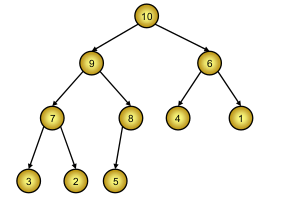
\includegraphics[scale=0.6]{img/heaptree.png}
\caption{Đống}
\label{HeapTree}
\end{figure}

\subsubsection{Vun đống}

Để biểu diễn dãy khóa arr[0...len-1] thành một cây nhị phân hoàn chỉnh. Giá trị arr[i] lưu trong nút thứ i (i bắt đầu từ 0). Nút con trái của nút thứ i là arr[2i+1] và con phải của nút thứ i là arr[2i+2]. Nút cha của nút thứ j là $(j-1) \% 2$.
\begin{figure}[htp]
\centering
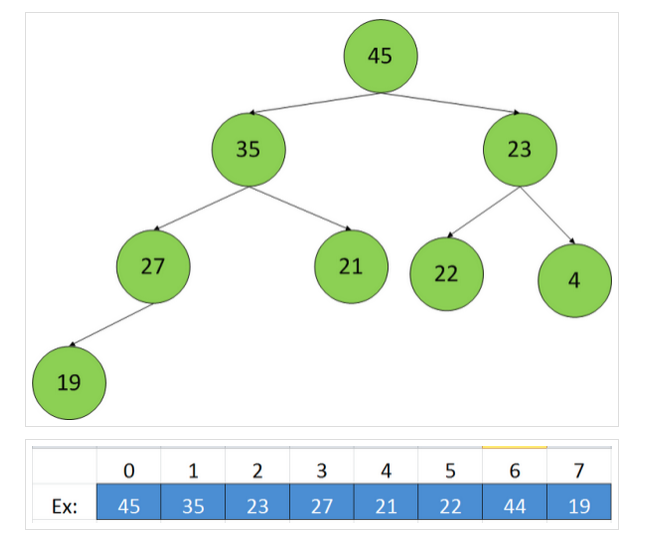
\includegraphics[scale=0.40]{img/bddong.png}
\caption{Biểu diễn đống bằng mảng}
\label{mangdong}
\end{figure}

Vì cây nhị phân gồm một nút thì hiển nhiên là đống. nên \textbf{để vun một nhánh cây gốc \texttt{r} thành đống, ta có thể coi hai nhánh con của nó là đống rồi và thực hiện thuật toán vun đống từ dưới lên đối với cây}. Gọi h là chiều cao của cây, nút ở mức h (nút lá) đã là một đống, ta vun lên những nút ở mức $h-1$ cũng là gốc của đống,... cứ như vậy cho tới mức 1 cũng là gốc của đống.

\paragraph{Thuật toán vun đống đối với gốc \texttt{r} khi hai nhánh con đã là đống}
Giả sử nút r chứa giá trị V. Tử r, ta cứ đi tới nút con chứa giá trị lớn nhất trong hai nút con, cho tới khi gặp phải một nút c mà mọi nút con của c đều có giá trị $ \le $ V (nút lá cũng là trường hợp riêng của điều kiện này). Dọc đường đi từ r tới c, ta đẩy giá trị chứa ở nút con lên nút cha và đặt giá trị V vào nút c.
\begin{figure}[htp]
\centering
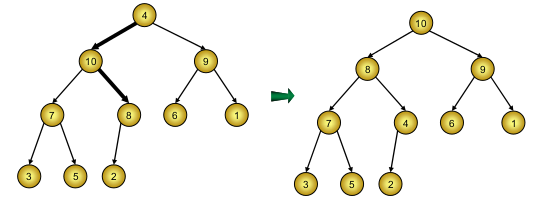
\includegraphics[scale=0.50]{img/buildheap.png}
\caption{Vun đống}
\label{}
\end{figure}

\subsubsection{Tư tưởng của Heap Sort}

Đầu tiên với dãy khóa arr[0...len-1] được vun từ dưới lên để nó biểu diễn một đống, khi đó khóa arr[0] tương ứng với nút gốc của đống là khóa lớn nhất, ta đảo giá trị khóa đó cho arr[len-1] và không tính tới arr[len-1] nữa. Còn lại dãy khóa arr[0...len-2] tuy không là đống nữa nhưng là biểu diễn của cây nhị phân hoàn chỉnh mà hai nhánh cây đã là đống rồi. Vậy chỉ cần vun một lần, ta lại dược một đống, đảo giá trị arr[0] với arr[len-2] rồi tiếp tục tới khi đống chỉ còn lại một nút.
\begin{figure}[htp]
\centering
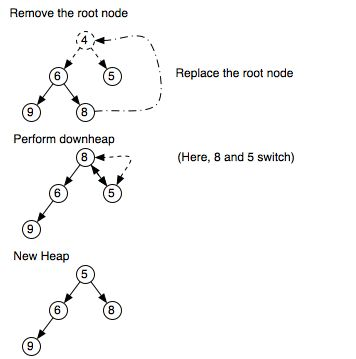
\includegraphics[scale=0.5]{img/tachdong.jpg}
\caption{Đảo giá trị của arr[0] và arr[len-1] rồi xét lại}
\label{}
\end{figure}

Thuật toán Heap Sort có hai hàm chính:

\begin{itemize}
\item Hàm \texttt{maxHeapify} làm nhiệm vụ vun cây gốc root thành đống trong điều kiện hai gốc con $2*root+1$ và $2*root+2$ đã là đống rồi. Các nút từ endnode+1 tới len-1 đã nằm đúng vị trí, không được tính tới nữa.
\item Hàm \texttt{heapSort} mô tả lại quá trình vun đống theo ý tưởng trên
\end{itemize}

\paragraph{Cài đặt}
\mnt{src/heapsort.cpp}

\paragraph{Độ phức tạp thuật toán}
Thuật toán sắp xếp \emph{Heap Sort} có độ phức tạp $n \log n $ trong mọi trường hợp.


\subsection{Đánh giá thời gian thực tế của thuật toán}Sau đây là một số kết quả chạy thử với các bộ dữ liệu đầu vào là các dãy sỗ được tạo ngẫu nhiên. Thời gian được tính theo đơn vị $ms$. 

\begin{figure}[htp]
\begin{center}
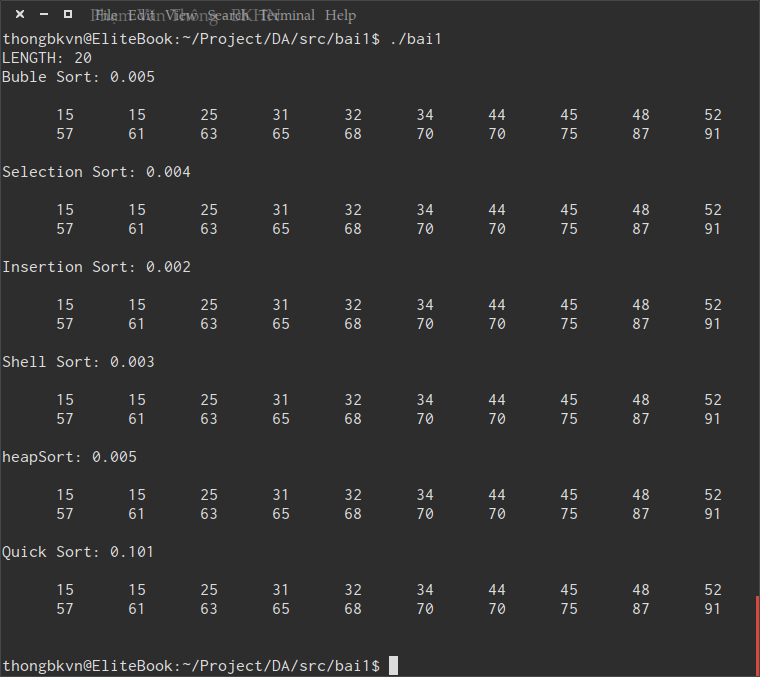
\includegraphics[scale=0.50]{img/bai1_20.png}
\caption{Dãy đầu vào có 20 phần tử}
\label{}
\end{center}
Trường hợp này, \emph{Quick Sort} chạy lâu nhất bởi có nhiều lời gọi đệ quy nhất. Tốc độ thực hiện kém xa các thuật toán khác.
\end{figure}

\begin{figure}[htp]
\begin{center}
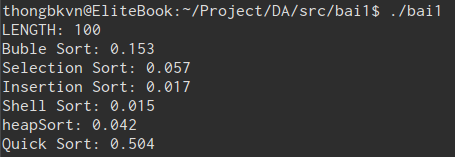
\includegraphics[scale=0.5]{img/bai1_100.png}
\caption{Dãy đầu vào có 100 phần tử.}
\label{}
\end{center}
\emph{Quick Sort} vẫn tỏ ra kém hơn so với các thuật toán khác. \emph{Buble Sort} bắt đầu tỏ ra chậm hơn so với \emph{Selection Sort} và \emph{Insertion Sort} do thực hiện nhiều phép tráo đổi.
\end{figure}

\begin{figure}[htp]
\begin{center}
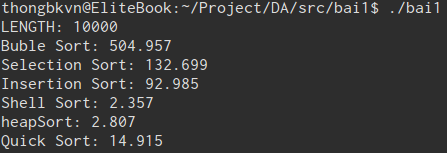
\includegraphics[scale=0.50]{img/bai1_10000.png}
\caption{Dãy đầu vào có 10 000 phần tử.}
\label{}
\end{center}
Các thuật toán sắp xếp \emph{Shell Sort}, \emph{Heap Sort}, \emph{Quick Sort} vượt trội hơn hẳn. \emph{Buble Sort} chậm nhất với $0.5s$.
\end{figure}

\begin{figure}[htp]
\begin{center}
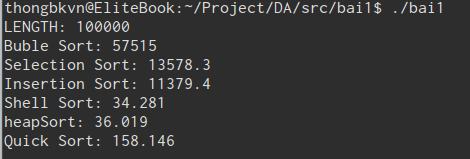
\includegraphics[scale=0.50]{img/bai1_100000.png}
\caption{Dãy đầu vào có 100 000 phần tử.}
\label{}
\end{center}
Các thuật toán sắp xếp như \emph{Buble Sort}, \emph{Selection Sort}, \emph{Insertion Sort} yếu kém hơn hẳn, ta sẽ không xét đến chúng trong ví dụ tới nữa. \emph{Shell Sort} và \emph{Heap Sort} vẫn rất ấn tượng với thời gian sắp xếp là $0.34s$.
\end{figure}

\begin{figure}[htp]
\begin{center}
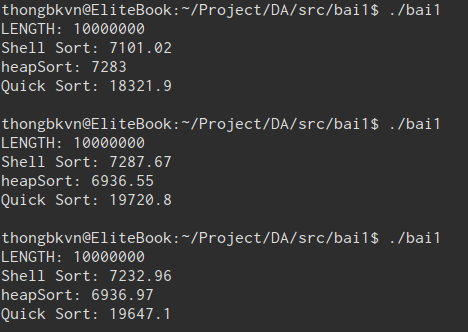
\includegraphics[scale=0.50]{img/bai1_10000000.png}
\caption{Dãy đầu vào có 10 000 000 phần tử.}
\label{}
\end{center}
\emph{Heap Sort} và \emph{Shell Sort} vẫn tỏ ra rất vượt trội.
\end{figure}
\newpage



\section{Các bài toán về thuật toán quay lui và kĩ thuật nhánh cận}
\subsection{Thuật toán quay lui}
Thuật toán quay lui dùng để giải bài toán \emph{liệt kê} các cấu hình. Mỗi cấu hình được xây dựng bằng cách xây dựng từng phần tử, mỗi phần tử được chọn bằng cách thử tất cả các khả năng. Giả sử cấu hình liệt kê có dạng X[1...n], khi đó thuật toán quay lui thực hiện qua các bước:
\begin{enumerate}
\item Xét tất cả các giá trị X[1] có thể nhận, thử cho X[1] nhận lần lượt các giá trị đó. Với mỗi giá trị thử gán cho X[1] ta sẽ:
\item Xét tất cả các giá trị X[2] có thể nhận, thử cho X[2] nhận lần lượt các giá trị đó. Với mỗi giá trị thử gán cho X[2] lại xét tiếp khả năng chọn X[3]... cứ tiếp tục như vậy đến bước:
\item Xét tất cả các giá trị X[n] có thể nhận, thử cho X[n] nhận lần lượt các giá trị đó, thông báo cầu hình tìm được (X[1], X[2], ... , X[n]).
\end{enumerate}

Trên phương diện quy nạp, có thể nói rằng thuật toán quay lui liệt kê các cấu hình n phần tử dạng X[1...n] bằng cách thử cho X[1] nhận lần lượt các giá trị có thể. Với mỗi giá trị thử gán cho X[1] bài toán trở thành liệt kê cấu hình n-1 phần tử sau X[2...n].\\

\textbf{Mô hình của thuật toán quay lui có thể mô tả như sau:}

\begin{verbatim}
void Try(int i)
{
    for (mọi giá trị V có thể gán cho X[i])
    {
        (Thử cho X[i] = V);
        if (X[i] là phần tử cuối cùng trong cấu hình)
        (thông báo cấu hình tìm được);
        else
        {
            (Ghi nhận việc X[i] đã được gán giá trị V);
            Try(i+1);
            (Nếu cần, bỏ việc ghi nhận X[i] = V để thử giá trị khác);
        }
    }
}
\end{verbatim}

Thuật toán quay lui sẽ bắt đầu bằng lời gọi Try(1) \footnote{Theo mô tả thuật toán quay lui ở đây thì sẽ bắt đầu với Try(1). Không phải các bài toán sử dụng thuật toán quay lui phảiluôn luôn bắt đầu bằng lời gọi Try(1), tùy theo việc cài đặt thuật toán.}
\subsection{Bài toán mã đi tuần}

\subsubsection{Bài toán}

Xét bàn cờ kích thước kích thước $N*N$. Một quân mã xuất phát tại vị trí (firstRow, firstCol). Quân mã phải đi theo đúng quy tắc bàn cờ vua và đi hết các ô trên bàn cờ sao cho mỗi ô đều được đi qua 1 lần.

\subsubsection{Cài đặt thuật toán}

Với bài toán này, ta sẽ giải quyết theo thuật toán quay lui. Bài toán sử dụng các biến và hàm sau:

\begin{description}
\item [Hằng N] Kích thước của bàn cờ.
\item [Biến firstRow, firstCol] Vị trí ban đầu của quân mã.
\item [Mảng A[N][N]] Lưu thứ tự các nước đi của quân mã, đồng thời cũng là mảng đóng vai trỏ đánh dầu khi ô tương ứng đã được đi qua. Vì vậy cần bỏ việc ghi nhận sau lời gọi đệ quy Try(i+1) để thử giá trị khác theo sơ đồ trên.
\item [Hàm printBoard()] In ra bàn cờ và thứ tự vị trí quân mã đã đi qua.
\item [Hàm Patrol] Hàm thực hiện quay lui để thử tất cả các cách đi quân mã trên bàn cờ có thể được và xuất kết quả ra màn hình nếu đi hết các ô.
\end{description}

\paragraph{Cài đặt thuật toán trên C++}
\mnt{src/knight.cpp}
\paragraph{Kết quả chạy thử}
\begin{figure}[htp]
\centering
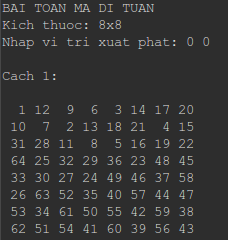
\includegraphics[scale=0.50]{img/knight1.png}
\caption{Kết quả chạy thử trên bàn cờ 8x8}
\label{}
\end{figure}

\subsection{Bài toán tám quân hậu}

\subsubsection{Bài toán}
\textbf{Bài toán tám quân hậu} là bài toán đặt tám \emph{quân hậu} trên bàn cờ vua kích thước 8x8 sao cho không có quân hậu nào có thể "ăn" được quân hậu khác. Như vậy, lời giải của bài toán là một cách xếp tám quân hậu trên bàn cờ sao cho không có hai quân nào đứng trên cùng hàng, hoặc cùng cột hoặc cùng đường chéo. Bài toán tám quân hậu có thể được tổng quát hóa thành bài toán N quân hậu.

\subsubsection{Cài đặt thuật toán}
Bài toán này cũng sẽ được giải quyết theo thuật toán quay lui. 


\paragraph{Phân tích}
Rõ ràng n quân hậu, mỗi con sẽ được đặt ở một hàng vì quân hậu được ăn ngang, ta gọi quân hậu sẽ đặt ở hàng 0 là quân hậu 0, quân hậu được đặt ở hàng 1 là quân hậu 1, quân hậu được đặt ở hàng n là quân hậu n. Như vậy, một nghiệm của bài toán sẽ được biết khi ta tìm ra được \textbf{vị trí cột của những quân hậu}.

Nếu ta định hướng Đông - Phải, Tây - Trái, Nam - Dưới, Bắc - Trên thì ta sẽ nhận thấy rằng:
\begin{itemize}
\item Một đường chéo theo hướng ĐB-TN bất kì sẽ đi qua một số ô, các ô đó có tính chất Hàng + Cột = C (hằng số). Với mỗi đường chéo ĐB-TN ta có một hằng số C và với một hằng số C: $0 \le C \le 2n-2$ xác định duy nhất một đường chéo ĐB-TN từ 0 đến 2n-2.
\item Một đường chéo hướng ĐN-TB bất kì đi qua một số ô, các ô có tính chất: Hàng - Cột = C. Với mỗi đường chéo ĐN-TB ta có một hằng số C và với một hằng số C: $-N+1 \le C \le N-1$ xác định duy nhất một đường chéo ĐN-TB.
\end{itemize}
\begin{figure}[htp]
\centering
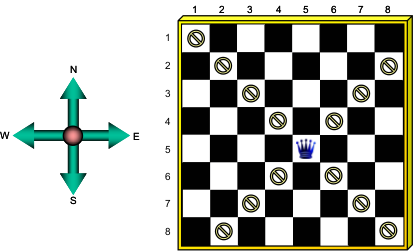
\includegraphics[scale=0.5]{img/quanhau.png}
\caption{Đường chéo ĐB-TN mang chỉ số 10 và đường chéo ĐN-TB mang chỉ số 0}
\label{}
\end{figure}

\paragraph{Cài đặt}
\begin{itemize}
\item Sử dụng 3 mảng để đánh dấu:
\begin{description}
\item [C[N]] $C[i] = 0$ nếu cột i còn tự do, $C[i] \neq 0$ nếu cột i đã bị một quân hậu khống chế.
\item [D1[2*N]] $D1[i] = 0$ nếu đường chéo DB-TN thứ i [ $0 \le i = row + col \le 2N$ ] còn tự do, $D1[i] \neq 0$ nếu đường chéo đó đã bị khống chế.
\item [D2[2*N]] $D2[i] = 0$ nếu đường chéo DN-TB thứ i [ $0 \le i = row - col + N - 1 \le 2N$ ] còn tự do, $D2[i] \neq 0$ nếu đã bị khống chế.
\end{description}
\item Sử dụng mảng A[N][N] để lưu kết quả.
\item Hàm \texttt{printBoard} dùng để xuất kết quả ra màn hình.
\item Hàm \texttt{Set} dùng để để đánh dấu và hủy đánh dấu các mảng đánh dấu khi thử đặt quân hậu vào vị trí hàng m, cột n. Tham số \texttt{unset} mặc định là 0 - bật đánh dấu. Nếu đặt bằng 1 sẽ là hủy đánh dấu.
\item Hàm checkBoard dùng để kiểm tra xem nước đi vào vị trí hàng i, cột j có đi được không bằng cách kiểm tra các mảng đánh dấu.
\item Hàm setBoard dùng giải thuật quay lui để thử tất cả các cách đặt quân hậu có thể được. Đây là chính trong bài toán này.
\end{itemize}

\paragraph {Cài đặt bài toán tám hậu trên C++}

\mnt{src/queen.cpp}

\paragraph {Kết quả chạy thử}
\begin{figure}[htp]
\centering
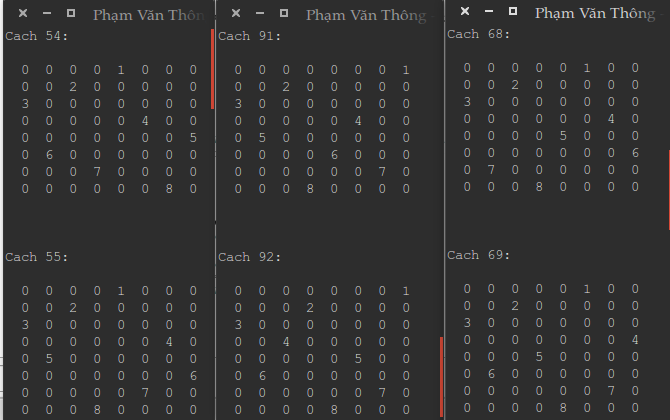
\includegraphics[scale=0.50]{img/queen.png}
\caption{Kết quả chạy thử}
\label{}
\end{figure}
\subsection{Bài toán người du lịch}

\subsubsection{Bài toán}
Có một người giao hàng cần đi giao hàng tại n thành phố. Anh ta xuất phát từ một thành phố nào đó, đi qua các thành phố khác để giao hàng và trở về thành phố ban đầu. Mỗi thành phố chỉ đến một lần, và khoảng cách từ một thành phố đến các thành phố khác đã được biết trước. Hãy tìm một chu trình (một đường đi khép kín thỏa mãn điều kiện trên) sao cho tổng độ dài các cạnh là nhỏ nhất.

\subsubsection{Cài đặt thuật toán}
\paragraph{Ý tưởng}

Hành trình cần tìm có dạng X[0...N], trong đó, $X[0] = X[N] = 0$, và ngoại trừ thành phố 0 là thành phố xuất phát thì không có thành phố nào được lặp lại 2 lần. Có nghĩ dãy X[1...N-1] lập thành một hoán vị của (1, 2, ..., N-1).

\textbf{Duyệt quay lui: } X[1] có thể chọn một trong các thành phố có thể đi từ X[0], với mỗi cách thử chọn X[1] như vậy thì chọn X[2] mà không trùng với X[0], ... Tổng quát: X[i] có thể chọn được các thành phố mà không trùng với các thành phố từ X[0] đến X[i-1].

\textbf{Nhánh cận:} Khởi tạo cấu hình \texttt{BestConfig} có chi phí $ +\infty $. Với mỗi bước thử chọn X[i] xem chi phí đường đi cho tới lúc đó có < chi phí của cấu hình BestConfig không. Nếu không nhỏ hơn thì thử giá trị khác ngay bởi có đi tiếp cũng chỉ tốn thêm. Khi thử được một giá trị X[N-1] thì đánh giá chi phí từ thành phố 1 đến thành phố X[N-1] cộng với chi phí từ X[N-1] về thành phố 0, nếu nhỏ hơn chi phí của đường đi ở BestConfig thì cập nhật lại BestConfig bằng cách đi mới.

\paragraph{Cài đặt}
\begin{itemize}
\item [Mảng X, BestWay] X ghi nhận đường đi trong quá trình thử, BestWay ghi nhận nghiệm.
\item [Mảng T, Free] Mảng T dùng để lưu tổng chi phi, T[i] là chi phí từ thành phố 0 tới thành phố i. Free dùng để đánh dấu thành phố đã được đi qua hay chưa.
\item [MinCost] Số tiền tối thiểu của chi phí đường đi trong BestConfig, khởi tạo với giá trị $100000$ biểu thị giá trị vô cùng lớn.
\item [findWay] Hàm quay lui thực hiện thử các khả năng. Tham số i biểu thị cho bước đi tới thành phố thứ i.
\end{itemize}

\paragraph{Cài đặt bài toán người du lịch trên C++}
\begin{description}
\item[Input] File văn bản "bai2.in".
\begin{itemize}
\item Dòng 1 chứa số N chỉ số lượng thành phố sẽ đi qua.
\item N dòng tiếp theo, mỗi dòng là một hàng gồm N số nguyên dương biểu thị ma trận chi phí A. Trong đó A[i][j] là chi phí đi từ thành phố i đến thành phố j. Ma trận A trong bài này là đối xứng.
\end{itemize}
\begin{figure}[htp]
\centering
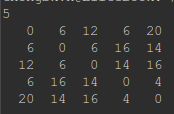
\includegraphics[scale=0.50]{img/bai2_dauvao.png}
\caption{Đầu vào từ file "bai2.in"}
\label{}
\end{figure}
\item [Output] Xuất ra màn hình lộ trình tìm được và chi phí của lộ trình.
\begin{figure}[htp]
\centering
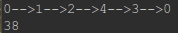
\includegraphics[scale=0.50]{img/bai2_daura.png}
\caption{Đầu ra chứa dãy biểu thị lộ trình và chi phí đường đi.}
\label{}
\end{figure}
\end{description}

\mnt{src/TSP.cpp}

\newpage

\section{Bài toán đánh chỉ mục cho danh sách từ khóa}

\subsection{Bài toán}
Có một file văn bản gồm danh sách các từ khóa và một file văn bản khác là tài liệu chứa các từ khóa đó. Viết chương trình lưu danh sách từ khóa và dòng xuất hiện của từ khóa đó trong tài liệu, cài đặt với các cấu trúc dữ liệu khác nhau: danh sách liên kết, bảng băm, cây nhị phân tìm kiếm.

\subsection{Ý tưởng}
Lưu các từ khóa trong các cấu trúc dữ liệu khác nhau - danh sách liên kết, bảng băm và cây nhị phân tìm kiếm.
\begin{figure}[htp]
\centering
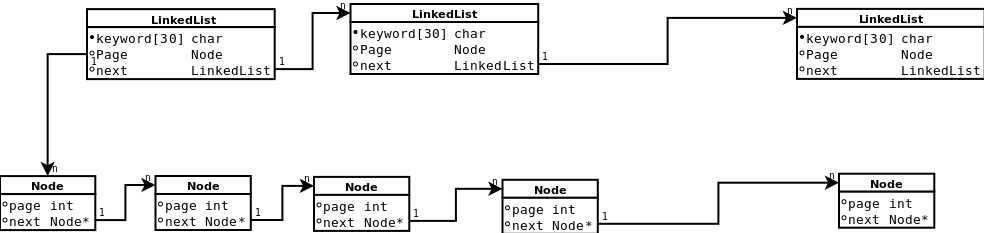
\includegraphics[scale=0.40]{img/Diagram1.png}
\caption{Danh sách liên kết chứa từ khóa.}
\label{}


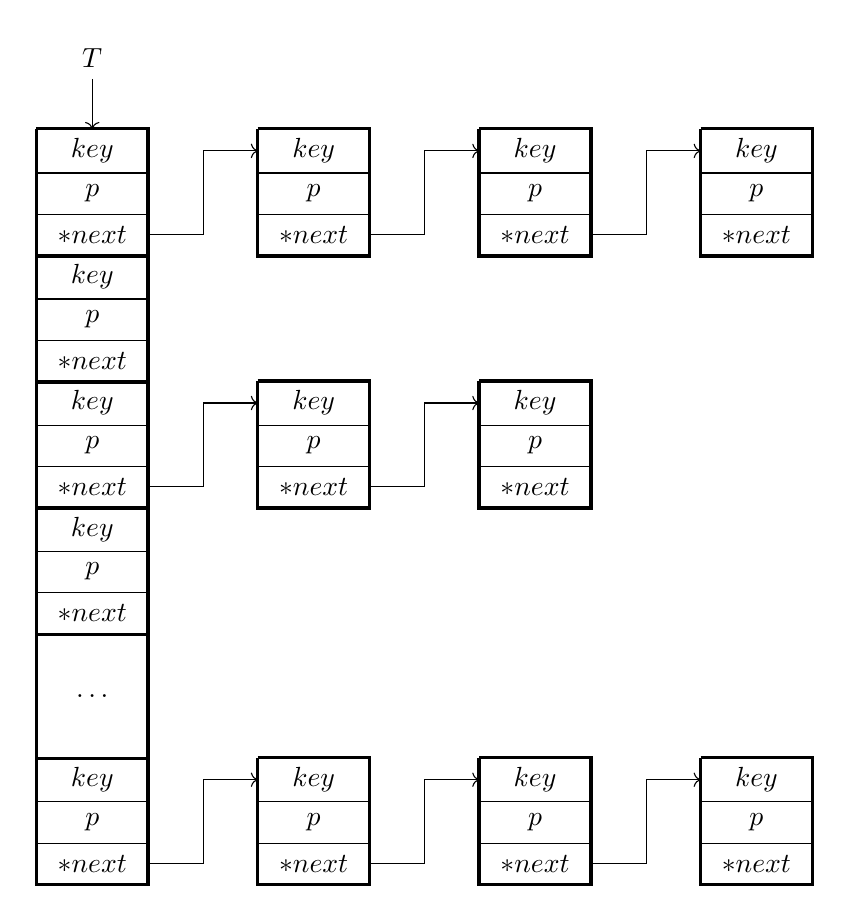
\begin{tikzpicture}[every node/.style={minimum height=1.5em,minimum width=4em}]
\matrix[matrix of math nodes](a)
{T & |[minimum width=4em]| & & |[minimum width=4em]| & & |[minimum width=4em]| & & \\
 |[minimum height=1.5em]|& & & & & & &\\
key & & key & & key & & key & \\
p & & p & & p & & p &\\
*next & & *next & & *next & & *next & \\
key & & & & & & & \\
p & & & & & & & \\
*next & & & & & & & \\
key & & key & & key & & &\\
p & & p & & p & & &\\
*next & & *next & & *next & & &\\
key & & & & & & & \\
p & & & & & & & \\
*next & & & & & & & \\
|[minimum height=4.5em]|\ldots & & & & & & & \\
key & & key & & key & & key &\\
p & & p & & p & & p & \\
*next & & *next & & *next & & *next & \\
};
\draw[very thick] (a-3-1.north west) -- (a-3-1.north east) -- (a-18-1.south east) -- (a-18-1.south west) -- (a-3-1.north west);
\draw (a-3-1.south west) -- (a-3-1.south east);
\draw (a-4-1.south west) -- (a-4-1.south east);
\draw[very thick] (a-5-1.south west) -- (a-5-1.south east);
\draw (a-6-1.south west) -- (a-6-1.south east);
\draw (a-7-1.south west) -- (a-7-1.south east);
\draw[very thick] (a-8-1.south west) -- (a-8-1.south east);
\draw (a-9-1.south west) -- (a-9-1.south east);
\draw (a-10-1.south west) -- (a-10-1.south east);
\draw[very thick] (a-11-1.south west) -- (a-11-1.south east);
\draw (a-12-1.south west) -- (a-12-1.south east);
\draw (a-13-1.south west) -- (a-13-1.south east);
\draw[very thick] (a-14-1.south west) -- (a-14-1.south east);
\draw[very thick] (a-15-1.south west) -- (a-15-1.south east);
\draw (a-16-1.south west) -- (a-16-1.south east);
\draw (a-17-1.south west) -- (a-17-1.south east);

\draw[very thick] (a-3-3.north west) -- (a-3-3.north east) -- (a-5-3.south east) -- (a-5-3.south west) -- (a-3-3.north west);
\draw (a-3-3.south west) -- (a-3-3.south east);
\draw (a-4-3.south west) -- (a-4-3.south east);

\draw[very thick] (a-3-5.north west) -- (a-3-5.north east) -- (a-5-5.south east) -- (a-5-5.south west) -- (a-3-5.north west);
\draw (a-3-5.south west) -- (a-3-5.south east);
\draw (a-4-5.south west) -- (a-4-5.south east);

\draw[very thick] (a-3-7.north west) -- (a-3-7.north east) -- (a-5-7.south east) -- (a-5-7.south west) -- (a-3-7.north west);
\draw (a-3-7.south west) -- (a-3-7.south east);
\draw (a-4-7.south west) -- (a-4-7.south east);

\draw[very thick] (a-9-3.north west) -- (a-9-3.north east) -- (a-11-3.south east) -- (a-11-3.south west) -- (a-9-3.north west);
\draw (a-9-3.south west) -- (a-9-3.south east);
\draw (a-10-3.south west) -- (a-10-3.south east);

\draw[very thick] (a-9-5.north west) -- (a-9-5.north east) -- (a-11-5.south east) -- (a-11-5.south west) -- (a-9-5.north west);
\draw (a-9-5.south west) -- (a-9-5.south east);
\draw (a-10-5.south west) -- (a-10-5.south east);

\draw[very thick] (a-16-3.north west) -- (a-16-3.north east) -- (a-18-3.south east) -- (a-18-3.south west) -- (a-16-3.north west);
\draw (a-16-3.south west) -- (a-16-3.south east);
\draw (a-17-3.south west) -- (a-17-3.south east);

\draw[very thick] (a-16-5.north west) -- (a-16-5.north east) -- (a-18-5.south east) -- (a-18-5.south west) -- (a-16-5.north west);
\draw (a-16-5.south west) -- (a-16-5.south east);
\draw (a-17-5.south west) -- (a-17-5.south east);

\draw[very thick] (a-16-7.north west) -- (a-16-7.north east) -- (a-18-7.south east) -- (a-18-7.south west) -- (a-16-7.north west);
\draw (a-16-7.south west) -- (a-16-7.south east);
\draw (a-17-7.south west) -- (a-17-7.south east);

\draw[->] (a-1-1.south) -- (a-3-1.north);

\draw[->] (a-5-1.east) -|++(1em,0em) coordinate(aa) --++(1em,0em)|- (a-3-3.west);
\draw[->] (a-5-3.east) -|++(1em,0em) coordinate(aa) --++(1em,0em)|- (a-3-5.west);
\draw[->] (a-5-5.east) -|++(1em,0em) coordinate(aa) --++(1em,0em)|- (a-3-7.west);

\draw[->] (a-11-1.east) -|++(1em,0em) coordinate(aa) --++(1em,0em)|- (a-9-3.west);
\draw[->] (a-11-3.east) -|++(1em,0em) coordinate(aa) --++(1em,0em)|- (a-9-5.west);

\draw[->] (a-18-1.east) -|++(1em,0em) coordinate(aa) --++(1em,0em)|- (a-16-3.west);
\draw[->] (a-18-3.east) -|++(1em,0em) coordinate(aa) --++(1em,0em)|- (a-16-5.west);
\draw[->] (a-18-5.east) -|++(1em,0em) coordinate(aa) --++(1em,0em)|- (a-16-7.west);
\end{tikzpicture}
\caption{Lưu các từ khóa vào bảng băm.}
\end{figure}
Với mỗi nút, ngoài mảng kí tự chứa từ khóa, ta còn lưu thêm một biến kiểu Node chính là \emph{Header} của danh sách liên kết, mà mỗi phần tử của danh sách liên kết là một số nguyên, biểu thị cho vị trí xuất hiện của từ khóa.

Đọc lần lượt từng dòng của \emph{tài liệu} cần đánh chỉ mục, với mỗi dòng, đọc được, ta lần lượt tìm kiếm các từ xuất hiện trong dòng đó xem có trùng với từ khóa được lưu trữ trong cấu trúc dữ liệu trước đó không, nếu trùng, thêm vị trí xuất hiện của từ khóa (số thứ tự dòng) vào danh sách liên kết có header là phần tử kiểu Node. Xem hình minh họa để hiểu rõ hơn chi tiết cài đặt.

\subsection{Cài đặt với danh sách liên kết}
\mnt{src/linkedlist.cpp}
\subsection{Cài đặt với bảng băm}
\mnt{src/hashtable.cpp}
\subsection{Cài đặt với cây nhị phân tìm kiếm}
\mnt{src/tree.cpp}
\subsection{Kết quả chạy thử}
\begin{figure}[htp]
\centering
\includegraphics[scale=0.3]{img/linklist_rs.png}
\caption{Phiên bản danh sách liên kết.}
\label{}
\end{figure}

\begin{figure}[htp]
\centering
\includegraphics[scale=0.3]{img/hashtable_rs.png}
\caption{Phiên bản bảng băm.}
\label{}
\end{figure}

\begin{figure}[htp]
\centering
\includegraphics[scale=0.3]{img/tree_rs.png}
\caption{Phiên bản cây nhị phân tìm kiếm.}
\label{}
\end{figure}












\end{document}